\documentclass[aspectratio=169,xcolor=svgnames]{beamer}
%\documentclass{beamer}
%%%CHOOSE ASPECT RATIO ABOVE%%%

% \usetheme{LU-spfaff}

\usepackage[utf8]{inputenc}
\usepackage[british]{babel}
\usepackage{grffile}
\usepackage{minted}
\usepackage{csquotes}
\usepackage{tikz}
\usepackage{libertine}
\usepackage{fancyvrb}

% \usefonttheme{serif}

\usetikzlibrary{tikzmark}
\usetikzlibrary {arrows.meta}
\usetikzlibrary{positioning}
\usetikzlibrary{decorations.pathmorphing, decorations.pathreplacing, decorations.shapes,}

\tikzstyle{every picture} += [remember picture]

\setminted[java]{autogobble=true,bgcolor=LightGray,linenos}
\setminted[python]{autogobble=true,bgcolor=LightGray,linenos}

\setmonofont{Fira Code}

\title[]{Bayesian Statistics}

% \titlecolor{LUGreen} % Choose between LUPink, LULBlue, LUIvory, LUGreen
%\titleimage{\includegraphics[scale=.5]{astro.png}}
% \titleimage{\includegraphics[scale=.6]{lumainb.jpg}}
\author{Noric Couderc}
% \subtitle{Subtitles are currently limited to one line}
\date{\today}
\institute{Lund University\\Department of Computer Science}

\AtBeginSection[]{
  \begin{frame}
  \vfill
  \centering
  \begin{beamercolorbox}[sep=8pt,center,shadow=true,rounded=true]{title}
    \usebeamerfont{title}\textbf{\insertsectionhead}\par%
  \end{beamercolorbox}
  \vfill
  \end{frame}
}

\setbeamertemplate{footline}[frame number]

\begin{document}

\maketitle

\begin{frame}{About Me}
  \begin{columns}
    \column{0.5\textwidth}
    My name is Noric

    \begin{itemize}
    \item 5th year PhD student
    \item From: Digne les Bains, France
    \item Topics: Dynamic program analysis, performance engineering
    \item Supervisors: Christoph Reichenbach, Emma Söderberg
    \end{itemize}

    \column{0.5\textwidth}
    \includegraphics[width=\columnwidth]{/home/noric/Pictures/moi.jpg}

  \end{columns}
\end{frame}

\section{Performance Example}

\begin{frame}
  \begin{figure}[ht]
    \centering
    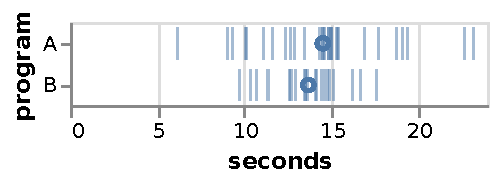
\includegraphics[width=\textwidth]{figures/samples_a_b.pdf}
    \caption{Which program is faster?}
  \end{figure}

\end{frame}

\begin{frame}{Normal Distribution}
  \begin{figure}[ht]
    \centering
    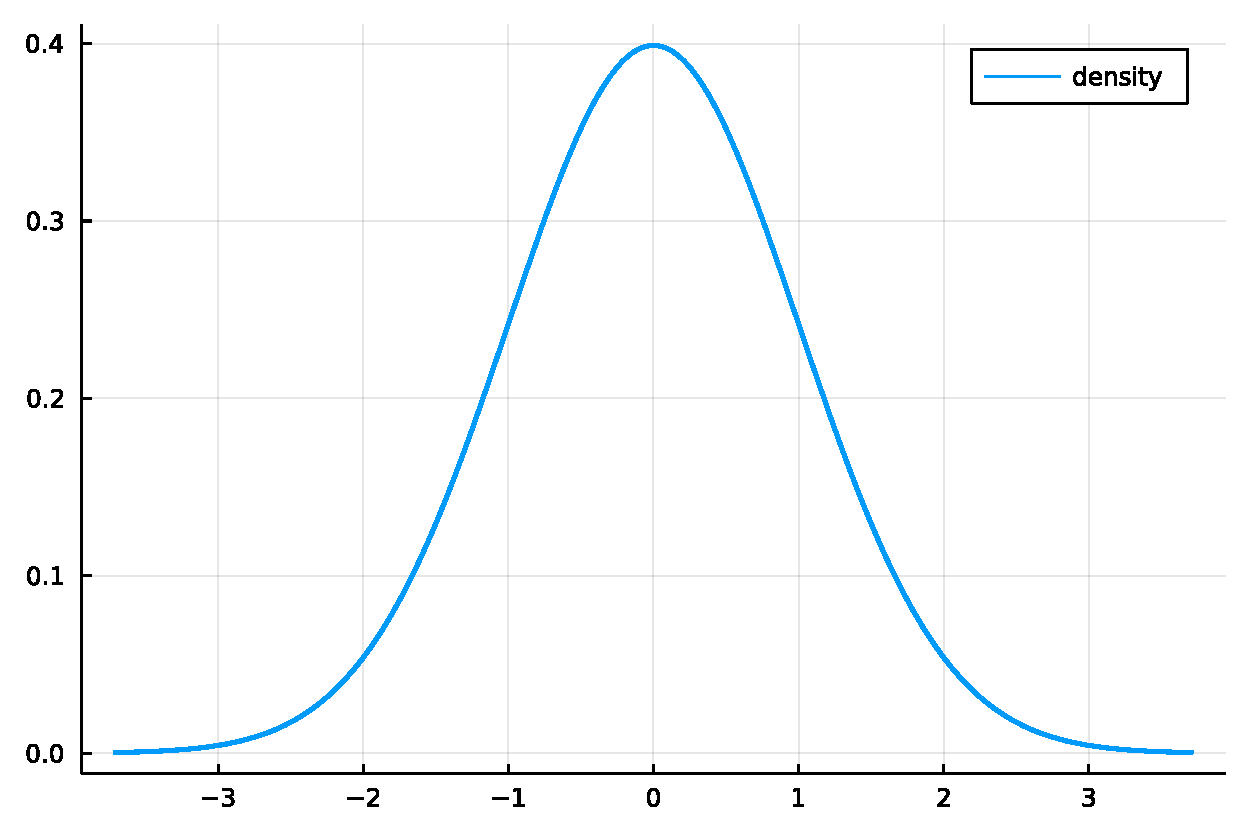
\includegraphics[width=0.8\textwidth]{figures/normal_distribution.pdf}
    % \caption{\label{fig:label} }
  \end{figure}
\end{frame}

\begin{frame}{Sampling}
  % Show ``the mean'' doesn't really exist, it has some error!
  \begin{figure}[ht]
    \centering
    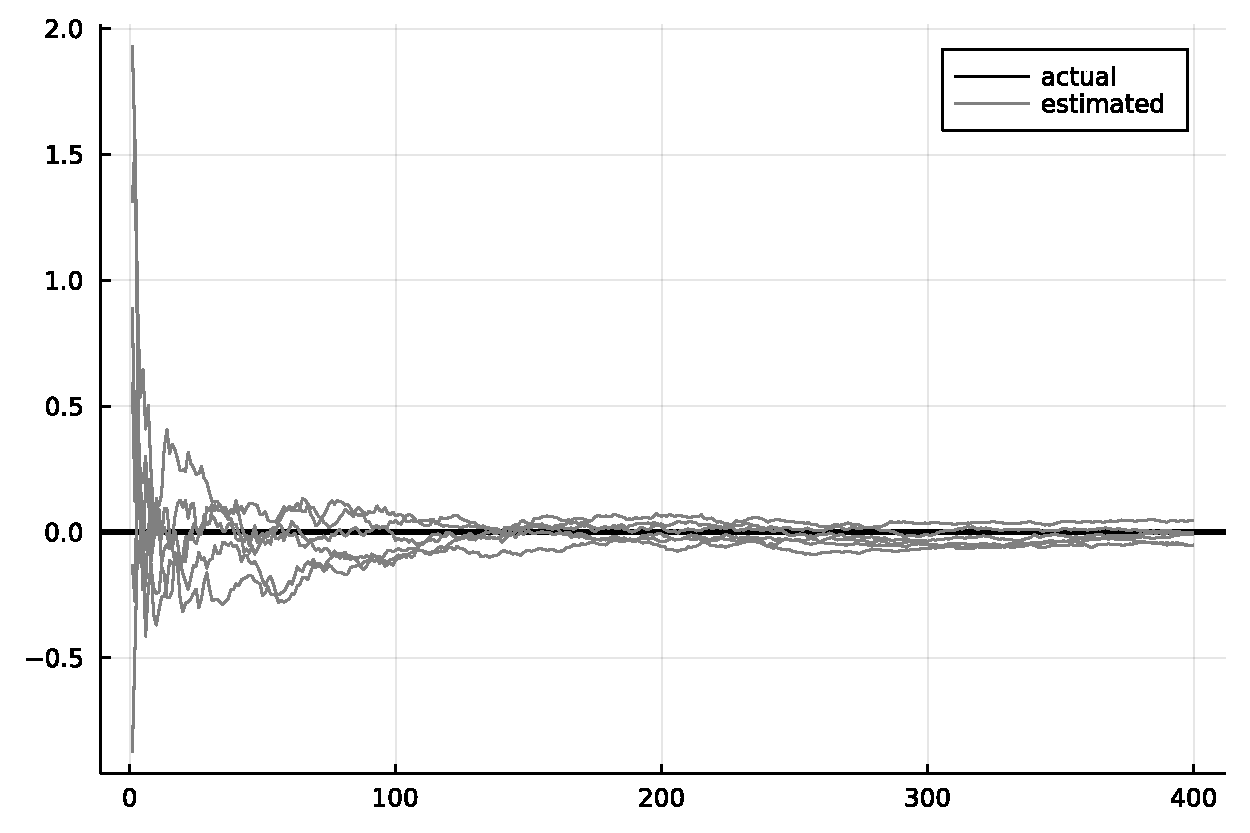
\includegraphics[width=0.8\textwidth]{figures/mean_error.pdf}
  \end{figure}
\end{frame}

\begin{frame}{Sampling}
  \begin{columns}
    \begin{column}{0.4\textwidth}
    \begin{figure}[ht]
        \centering
        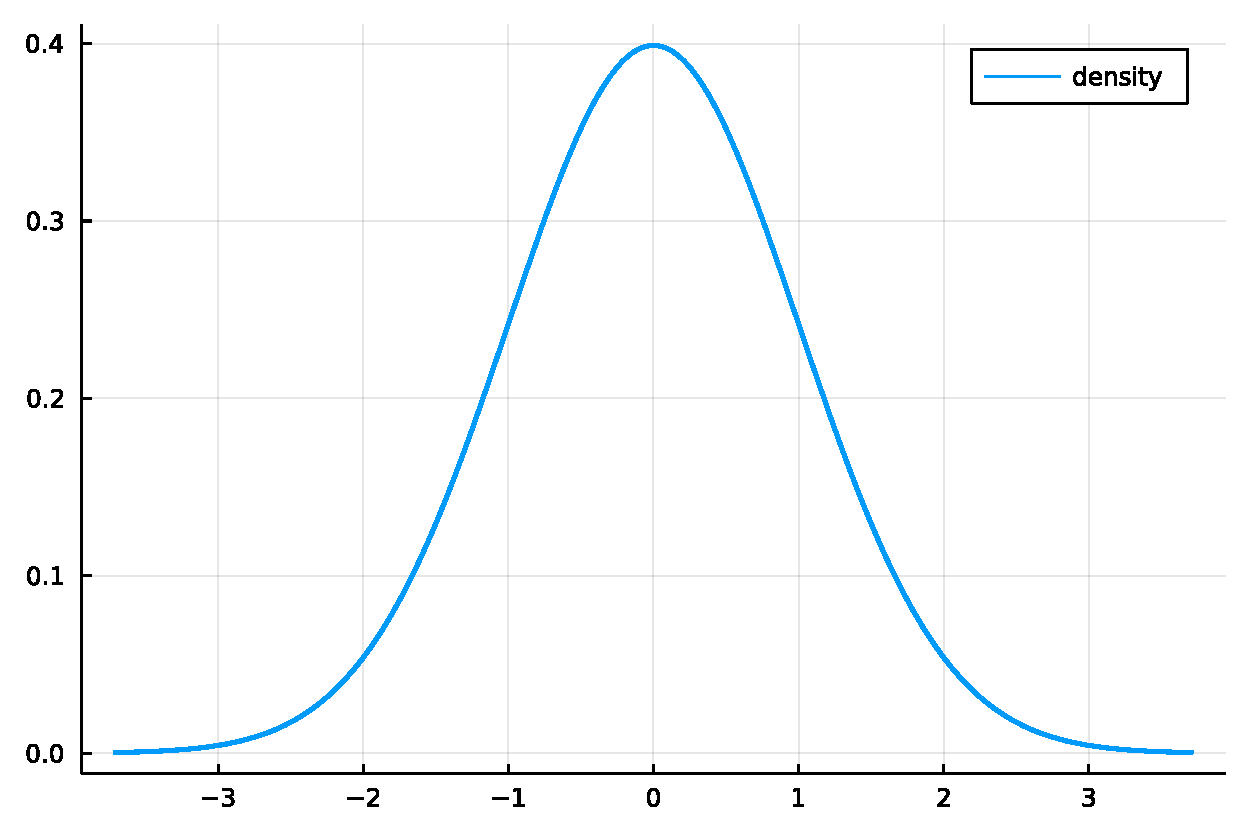
\includegraphics[width=\textwidth]{figures/normal_distribution.pdf}
        % \caption{\label{fig:label} }
    \end{figure}
    \end{column}
    \begin{column}{0.6\textwidth}
      \begin{figure}[ht]
        \centering
        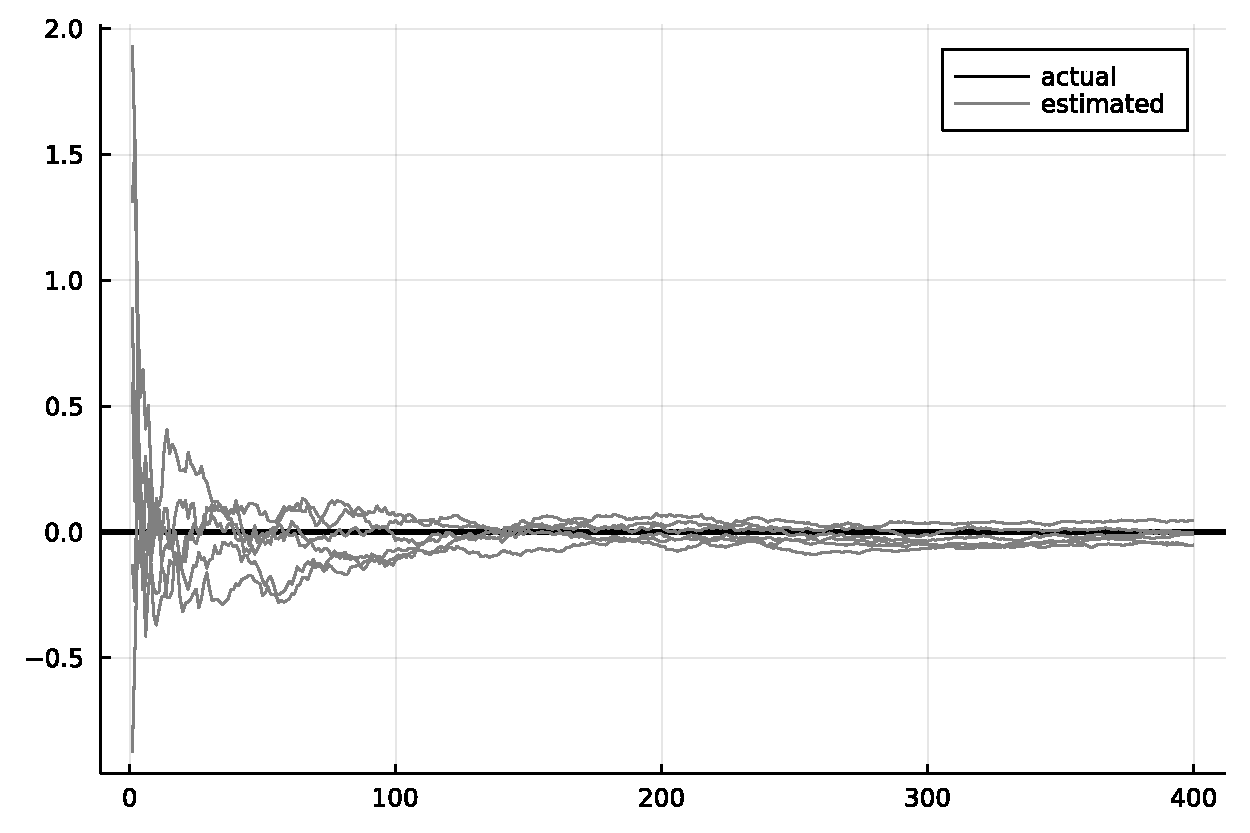
\includegraphics[width=\textwidth]{figures/mean_error.pdf}
      \end{figure}
    \end{column}
  \end{columns}
\end{frame}

\begin{frame}
  \huge
  \center
  Statistics

  Working with numbers you \textbf{can't trust}
\end{frame}

\begin{frame}
  \begin{columns}
    \begin{column}{0.5\textwidth}
      \center
      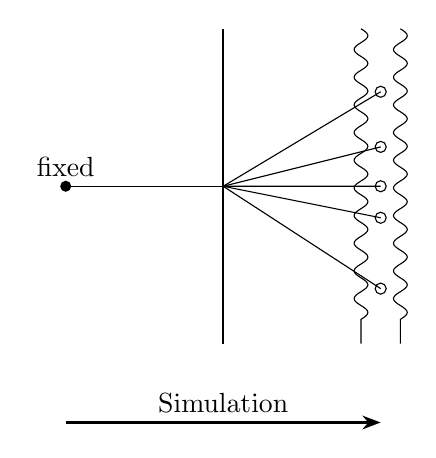
\begin{tikzpicture}[>=Stealth]
        \draw[thick] (0, 2) -- (0, -2);
        \fill (-2, 0) circle[radius=2pt] node[above] {fixed};

        \draw (-2, 0) -- (0, 0);

        \draw (0,0) -- (2,0) circle[radius=2pt] ;
        \draw (0,0) -- (2,0.5) circle[radius=2pt] ;
        \draw (0,0) -- (2,-0.4) circle[radius=2pt] ;
        \draw (0,0) -- (2,1.2) circle[radius=2pt] ;
        \draw (0,0) -- (2,-1.3) circle[radius=2pt] ;

        \draw[decorate, decoration={coil, aspect=0}] (1.75, 2) -- (1.75,-2);
        \draw[decorate, decoration={coil, aspect=0}] (2.25, 2) -- (2.25,-2);

        \draw[->,thick] (-2, -3) -- node[midway,above] {Simulation} (2, -3);
      \end{tikzpicture}
    \end{column}
    \begin{column}{0.5\textwidth}
      \center
      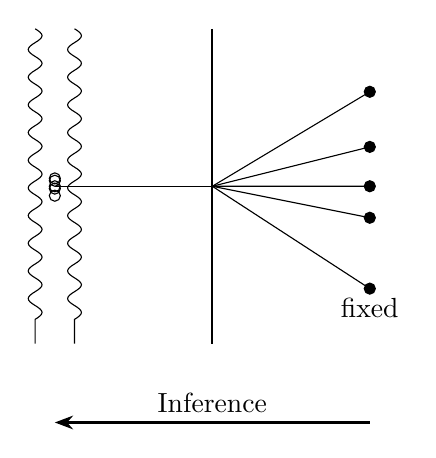
\begin{tikzpicture}[>=Stealth]
        \draw[thick] (0, 2) -- (0, -2);
        \draw(-2, 0) circle[radius=2pt];
        \draw(-2, 0.1) circle[radius=2pt];
        \draw(-2, 0.07) circle[radius=2pt];
        \draw(-2, -0.03) circle[radius=2pt];
        \draw(-2, -0.12) circle[radius=2pt];

        \draw (-2, 0) -- (0, 0);

        \draw[decorate, decoration={coil, aspect=0}] (-1.75, 2) -- (-1.75,-2);
        \draw[decorate, decoration={coil, aspect=0}] (-2.25, 2) -- (-2.25,-2);

        \draw[fill=black] (2,0) circle[radius=2pt] -- (0,0);
        \draw[fill=black] (2,0.5) circle[radius=2pt] -- (0,0);
        \draw[fill=black] (2,-0.4) circle[radius=2pt] -- (0,0);
        \draw[fill=black] (2,1.2) circle[radius=2pt] -- (0,0);
        \draw[fill=black] (2,-1.3) circle[radius=2pt] node[below] {fixed} -- (0,0);


        \draw[->,thick] (2, -3) -- node[midway,above] {Inference} (-2, -3);
      \end{tikzpicture}
    \end{column}
  \end{columns}
\end{frame}

\section{Maximum Likelihood Estimation}

\begin{frame}{Likelihood}
  \begin{equation*}
    P(\text{observed data}|\text{(hidden) parameters})
  \end{equation*}
\end{frame}

\begin{frame}{MLE Example}
Biased coin example.

(Maybe use Venus instead (cloud mask the sea!))
\end{frame}

\begin{frame}{Maximum Likelihood Estimation}
  \begin{itemize}
  \item Flexible!
  \item Needs some computational tricks (log-probabilities)
  \item Returns \emph{one single value}
  \item What if little data?
  \end{itemize}
\end{frame}

\section{Bayesian Statistics}

\begin{frame}
  \center
  What does a probability \textbf{mean}?
\end{frame}

\begin{frame}{Frequentist and Bayesian}
  \begin{block}{Frequentist}
    If I flip a coin for an \textbf{infinite number of times},
    half of the flips will turn heads.
  \end{block}

  \begin{block}{Bayesian}
    I do not know which side the coin I will see,
    so I say they have \textbf{equal chances}.
  \end{block}
\end{frame}

\begin{frame}
  \begin{itemize}
  \item Bayes theorem
  \item Prior distribution
  \item Likelihood
  \item Posterior distribution
  \end{itemize}

  (Use the hot/cold metaphor)
\end{frame}

\begin{frame}{Bayes' Rule}
  \begin{equation*}
    \tikz[baseline]{\node[anchor=base] (pab) {$P(A) \times P(B|A)$}}
    =
    \tikz[baseline]{\node[anchor=base] (pba) {$P(B) \times P(A|B)$}}
  \end{equation*}
  \begin{tikzpicture}[overlay, thick]
    \node<2->[above=of pab.north] (exp)  {$P(A \cap B)$};
    \node<2->[above=of pba.north] (exp1) {$P(B \cap A)$};
    % \node at (0, 1) {Other explanation};

    \draw<2-> (exp) -- (pab);
    \draw<2-> (exp1) -- (pba);
  \end{tikzpicture}

\end{frame}

\newcommand{\markmath}[2]{\tikz[baseline]{\node[anchor=base] (#1) {$#2$}}}

\begin{frame}{Bayes' Rule}
\begin{equation*}
  \markmath{posterior}{P(H|E)}
  =
  \frac{\markmath{prior}{P(H)} \times \markmath{likelihood}{P(E|H)}} {\markmath{norm}{P(E)}}
\end{equation*}

\begin{tikzpicture}[overlay, thick,>=Stealth]
  \node<2->[above left=of prior] (priorlabel) {Prior};
  \node<3->[above right=of likelihood] (liklabel) {Likelihood};
  \node<4->[left=of posterior] (postlabel) {Posterior};
  \node<5->[below=of norm] (normlabel) {Normalization};


  \draw<2->[->] (priorlabel) -- (prior);
  \draw<3->[->] (liklabel) -- (likelihood);
  \draw<4->[->] (postlabel) -- (posterior.west);
  \draw<5->[->] (normlabel) -- (norm);
\end{tikzpicture}
\end{frame}

\begin{frame}{Bayes' Rule}
  \begin{equation*}
    P(H|E) \propto P(H) \times P(E|H)
  \end{equation*}
\end{frame}

\begin{frame}
  \begin{itemize}
  \item Flexible!
  \item Needs some computational tricks too
  \item Returns distributions
  \item Works with little data
  \end{itemize}
\end{frame}

\section{Linear regression}

\begin{frame}
  \begin{itemize}
  \item Bayesian linear regression
  \item Interactions
  \item Counterfactual plots
  \item Prior sensitivity analysis
  \end{itemize}
\end{frame}

\begin{frame}
\begin{figure}[ht]
  \centering
  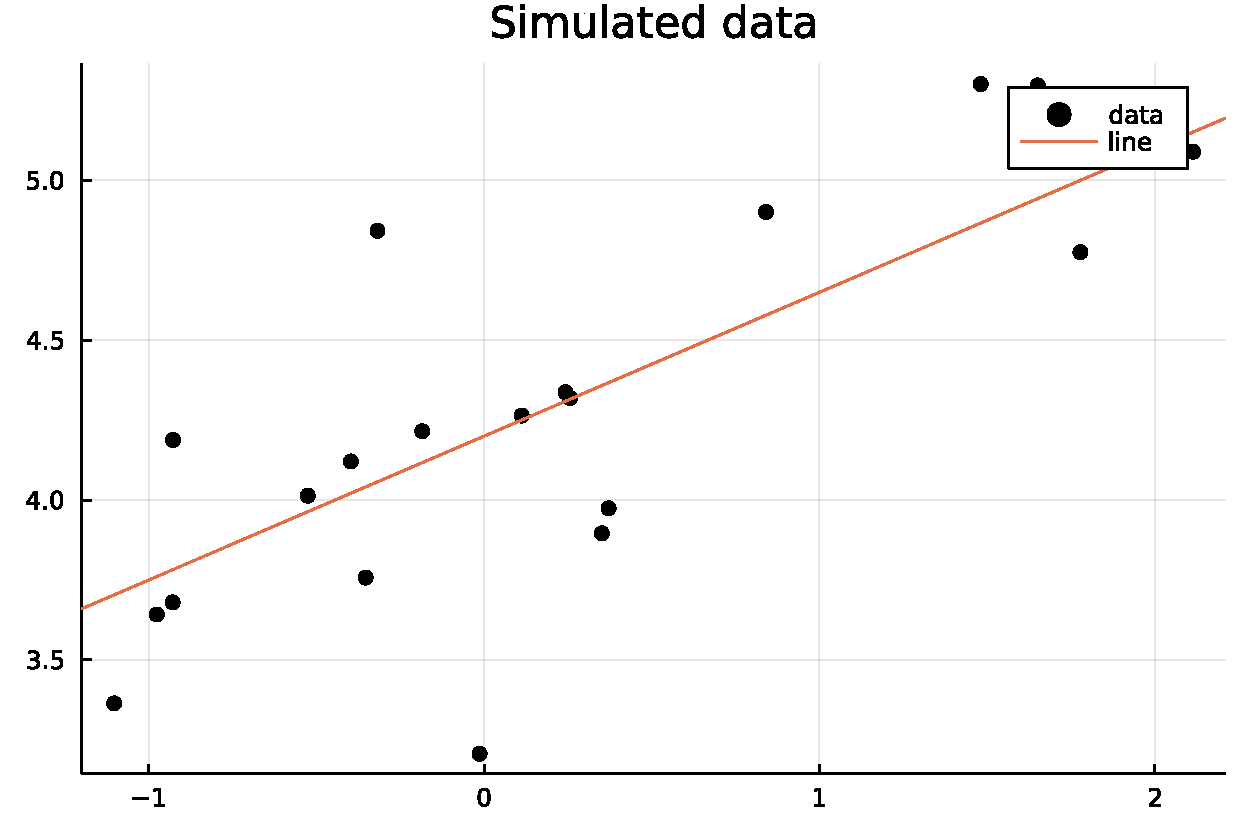
\includegraphics[width=0.8\textwidth]{figures/linear_data.pdf}
  \caption{\label{fig:label} Simulated data}
\end{figure}
\end{frame}

\begin{frame}
  \begin{figure}[ht]
    \centering
    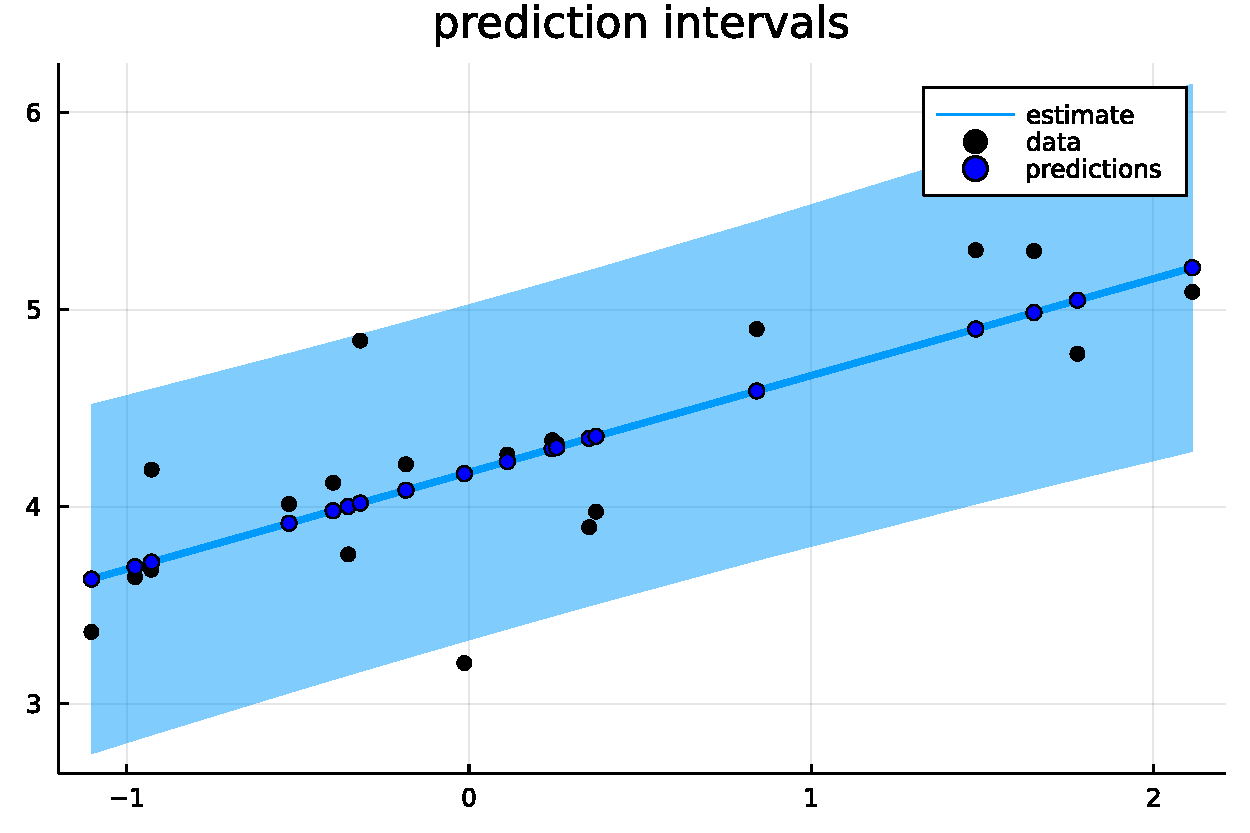
\includegraphics[width=0.8\textwidth]{figures/linear_prediction_interval.pdf}
    \caption{\label{fig:label} }
  \end{figure}
\end{frame}

\begin{frame}
  \begin{figure}[ht]
    \centering
    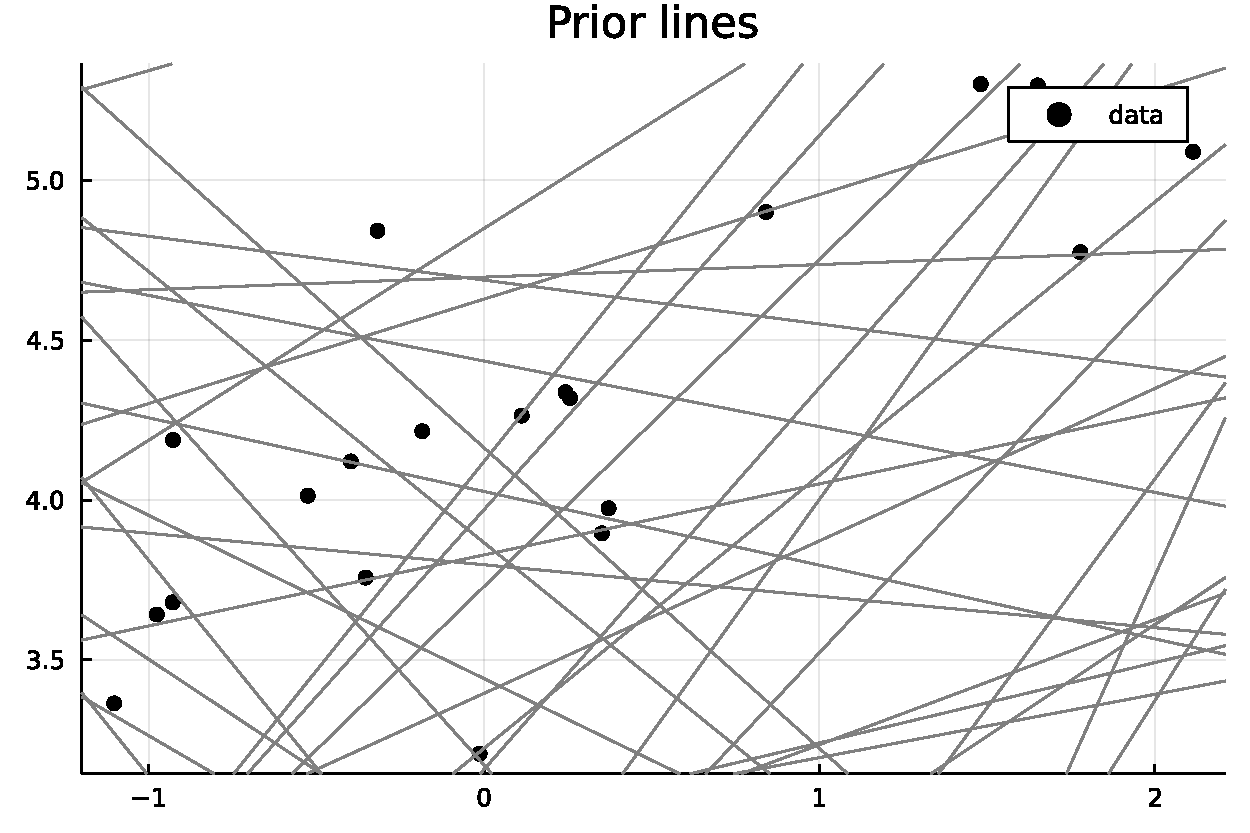
\includegraphics[width=0.8\textwidth]{figures/linear_prior_lines.pdf}
    \caption{\label{fig:label} }
  \end{figure}
\end{frame}

\begin{frame}
  \begin{figure}[ht]
    \centering
    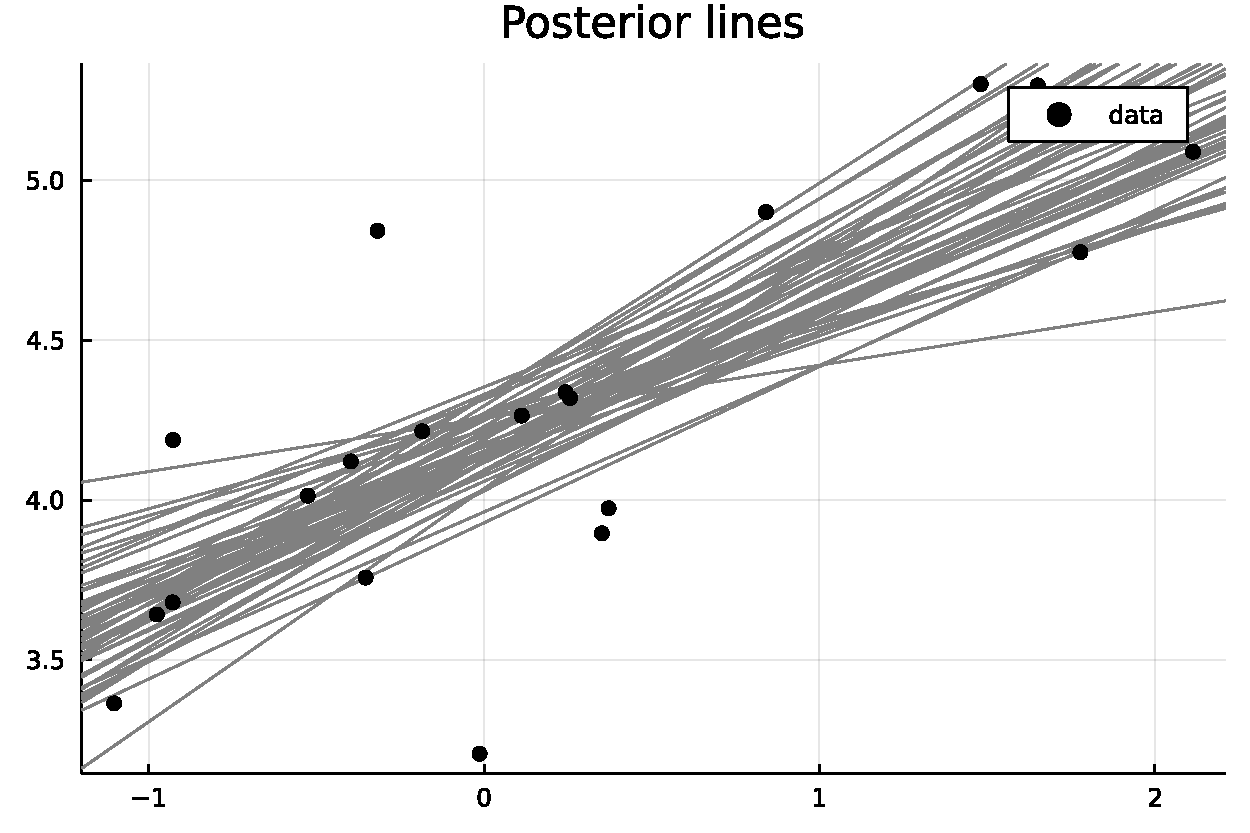
\includegraphics[width=0.8\textwidth]{figures/posterior_lines.pdf}
    \caption{\label{fig:label} }
  \end{figure}
\end{frame}

\begin{frame}
\begin{figure}[ht]
  \centering
  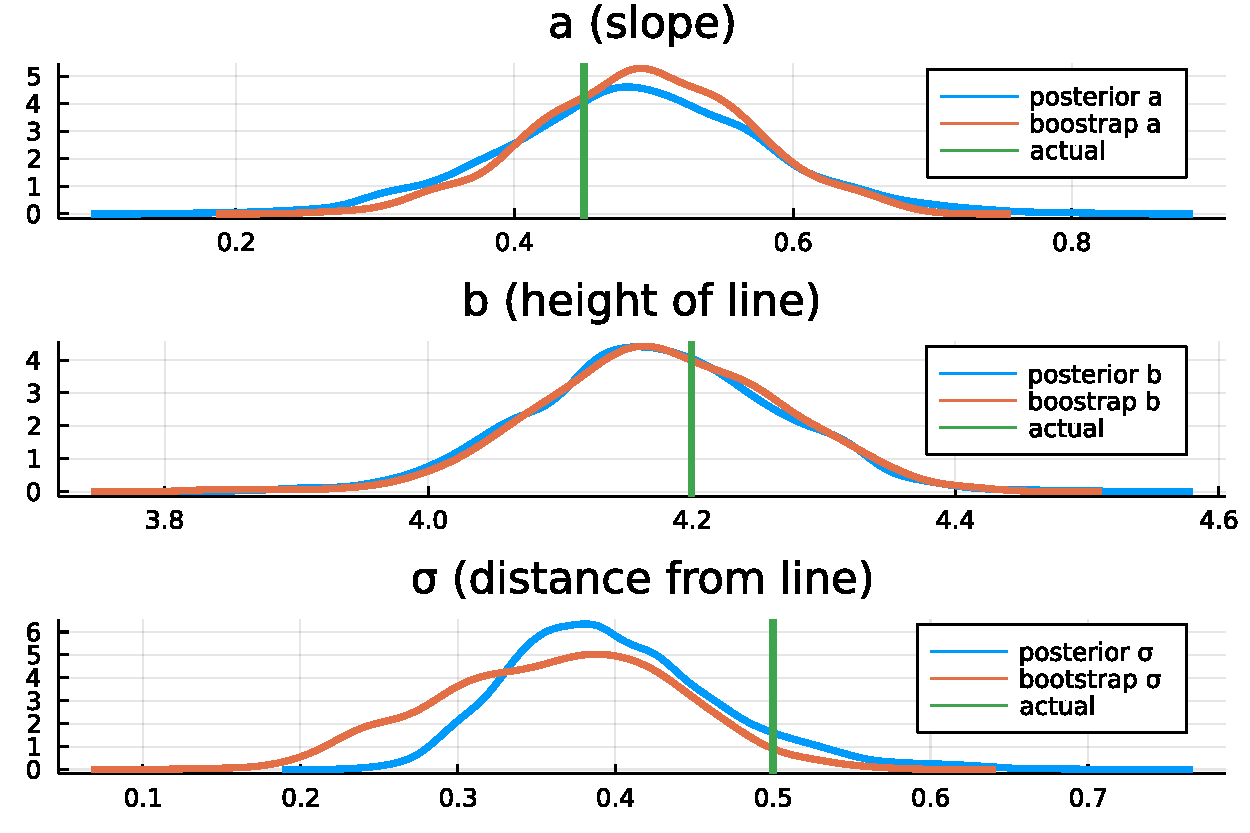
\includegraphics[width=0.8\textwidth]{figures/posterior_parameters.pdf}
  \caption{\label{fig:label} }
\end{figure}
\end{frame}

\begin{frame}
\begin{figure}[ht]
  \centering
  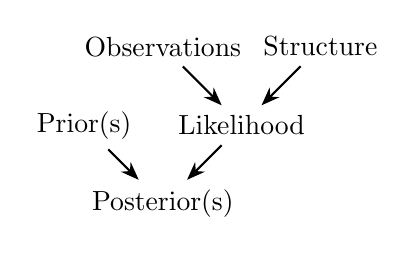
\begin{tikzpicture}[thick,>=Stealth]
    \node (priors) at (-1, 1) {Prior(s)};
    \node (posteriors) at (0,0) {Posterior(s)};
    \node (likelihood) at (1,1) {Likelihood};
    \node (data) at (0,2) {Observations};
    \node (structure) at (2,2) {Structure};

    \draw[->] (priors) -- (posteriors);
    \draw[->] (likelihood) -- (posteriors);
    \draw[->] (data) -- (likelihood);
    \draw[->] (structure) -- (likelihood);
  \end{tikzpicture}
\end{figure}
\end{frame}

\section{Posterior predictive simulation}

\begin{frame}
  \huge
  \center
  Predictions return \emph{distributions} too!
\end{frame}

\begin{frame}
\begin{figure}[ht]
  \centering
  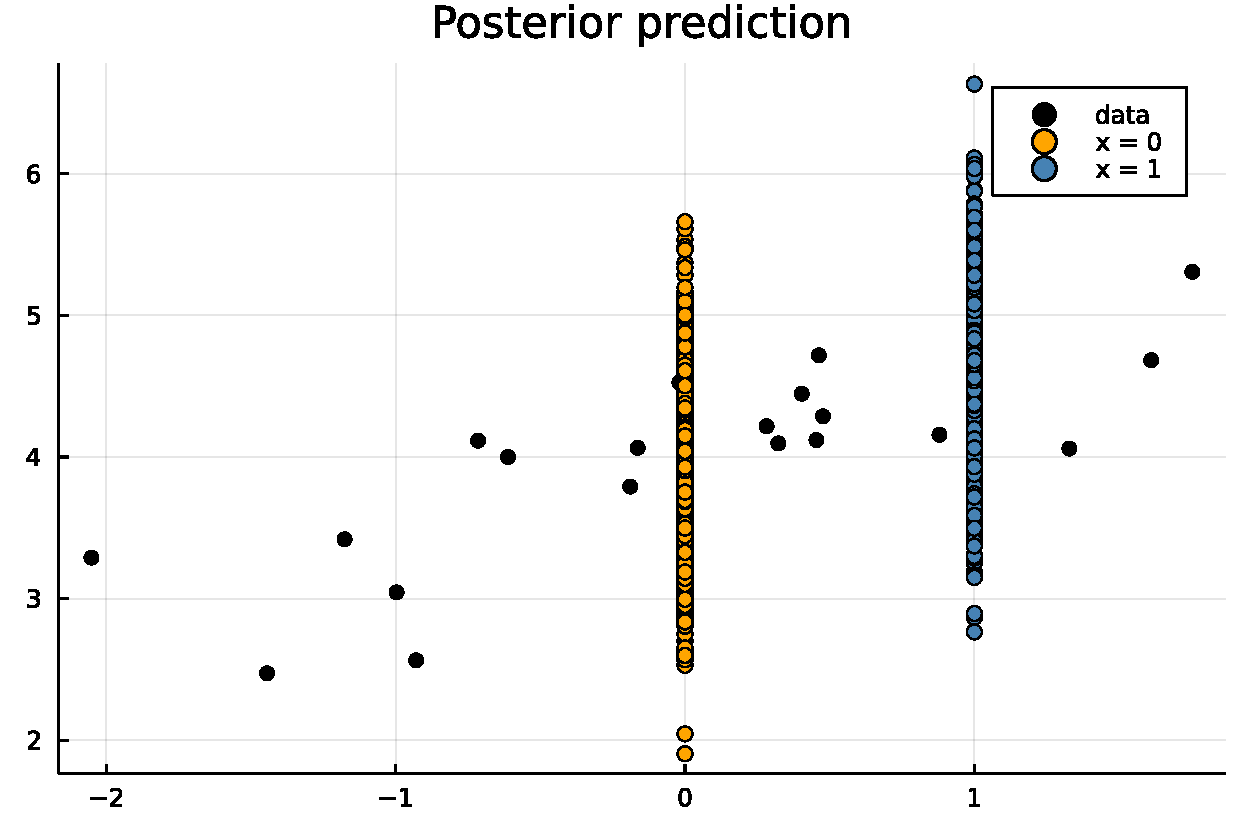
\includegraphics[width=0.8\textwidth]{figures/predictions.pdf}
\end{figure}
\end{frame}

\begin{frame}
\begin{figure}[ht]
  \centering
  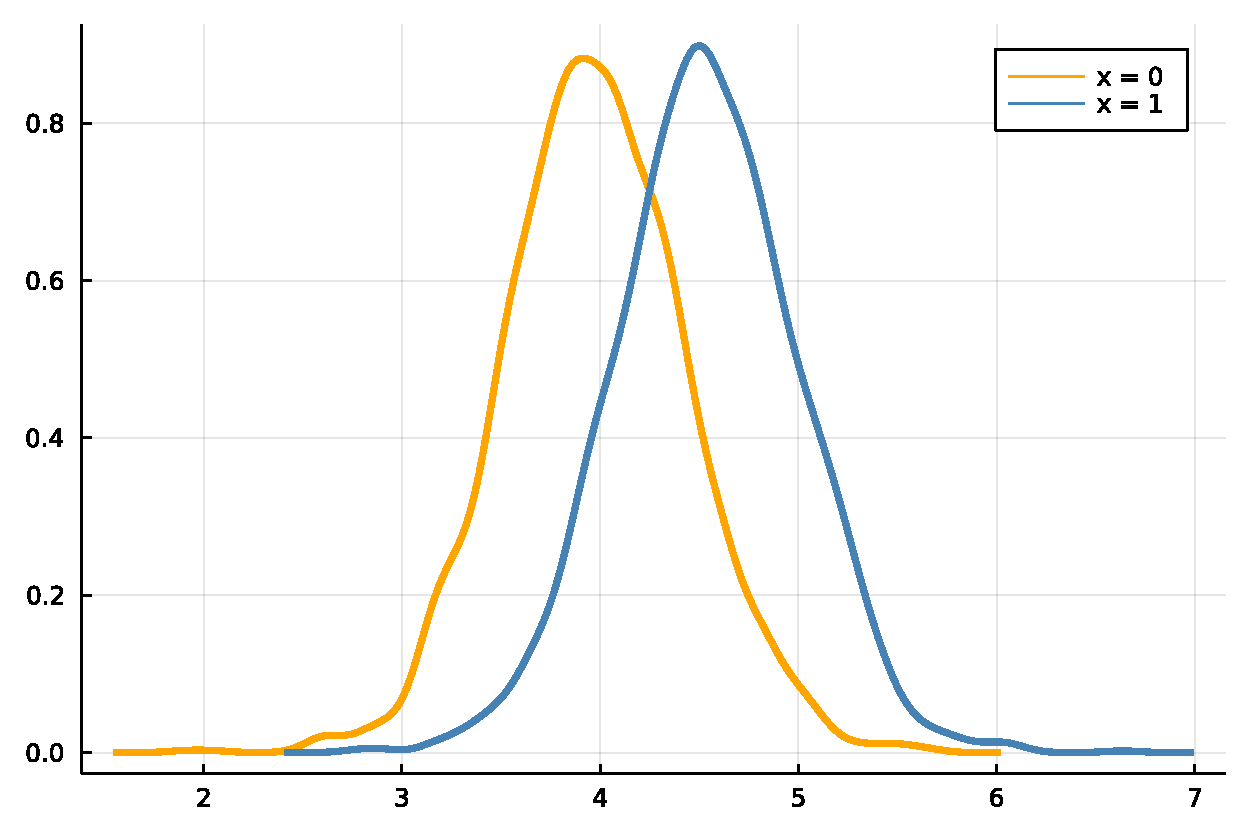
\includegraphics[width=0.8\textwidth]{figures/prediction_distrubtions.pdf}
\end{figure}
\end{frame}

\begin{frame}
\begin{figure}[ht]
  \centering
  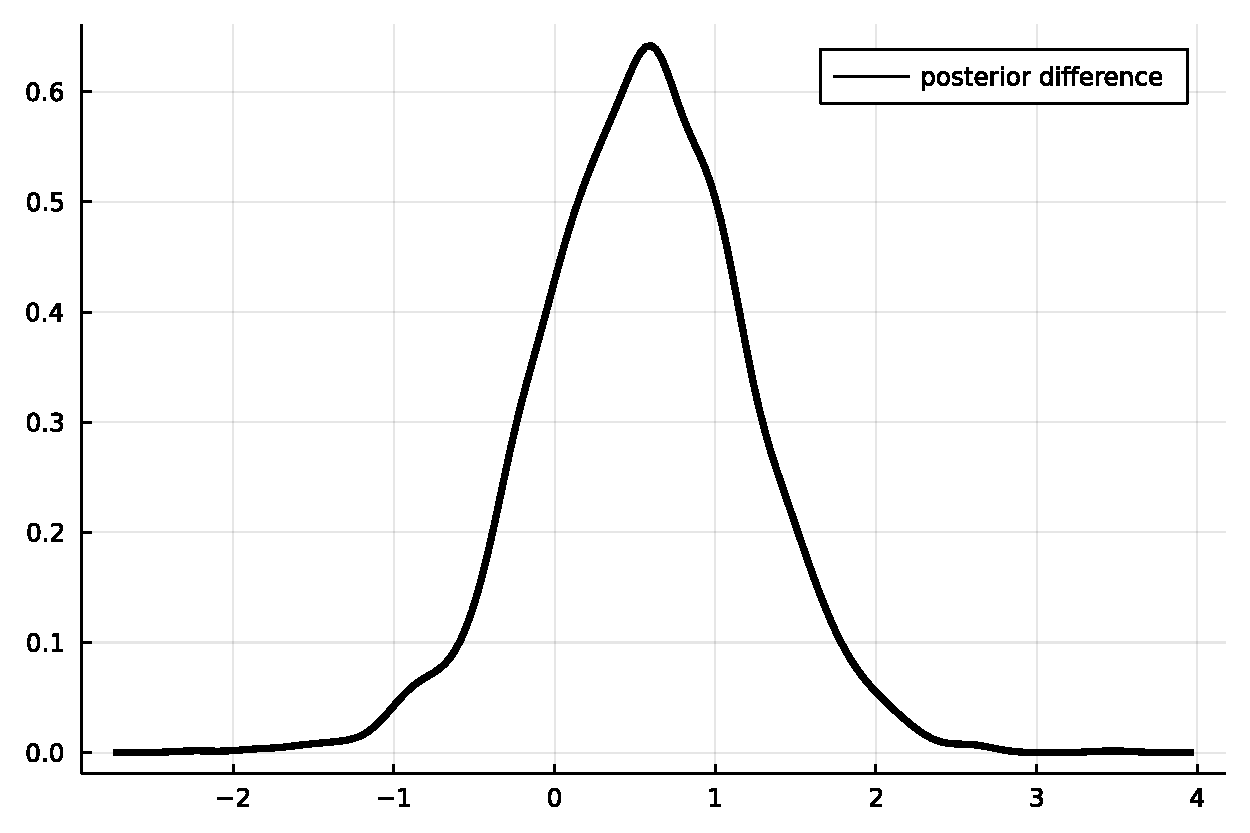
\includegraphics[width=0.8\textwidth]{figures/prediction_difference.pdf}
\end{figure}
\end{frame}

\section{Analysing Experiments}

\begin{frame}
  \center
  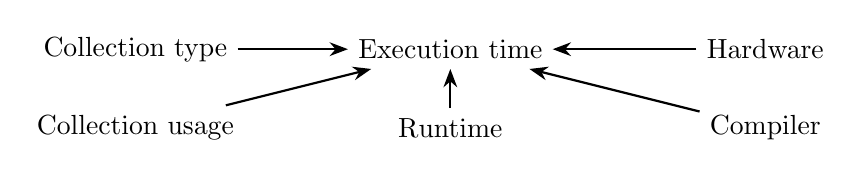
\begin{tikzpicture}[thick,>=Stealth]
    \node[] (collection) at (-4,1.0) {Collection type};
    \node[] (perf) at (0,1.0) {Execution time};
    \node[] (hardware) at (4,1.0) {Hardware};
    \node[] (usage) at (-4,0) {Collection usage};
    \node[] (compiler) at (4,0) {Compiler};
    \node[] (runtime) at (0,0) {Runtime};

    \draw[->] (collection) -- (perf.west);
    \draw[->] (usage) -- (perf);
    \draw[->] (hardware.west) -- (perf.east);
    \draw[->] (runtime) -- (perf);
    \draw[->] (compiler) -- (perf);
  \end{tikzpicture}
\end{frame}

\begin{frame}
  \center
  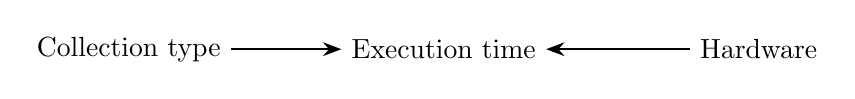
\begin{tikzpicture}[thick,>=Stealth]
    \node[] (collection) at (-4,1.0) {Collection type};
    \node[] (perf) at (0,1.0) {Execution time};
    \node[] (hardware) at (4,1.0) {Hardware};

    \draw[->] (collection) -- (perf.west);
    \draw[->] (hardware.west) -- (perf.east);
  \end{tikzpicture}
\end{frame}

\begin{frame}
  \begin{align*}
    \log(ET_j) &\sim \text{Normal}(\mu, \sigma)\\
    \mu &= \alpha[M_j] + \markmath{arrayaccess}{\beta[C_j]}\\
    \markmath{alpha}{\alpha_i} &\sim \text{Normal}(0.0, 0.5)\\
    \markmath{beta}{\beta_i} &\sim \text{Normal}(0.0, 0.2)\\
    \sigma &\sim \text{Exponential}(1.0)\\
  \end{align*}

  \begin{tikzpicture}[overlay, thick, >=Stealth]
    \node<2->[right=2cm of arrayaccess] (arrayaccesslabel) {Array access};
    \draw<2->[->] (arrayaccesslabel) -- (arrayaccess);

    \node<3->[left=2cm of alpha] (alphalabel) {Arrays};
    \draw<3->[->] (alphalabel) -- (alpha);
    \draw<3->[->] (alphalabel) -- (beta);
  \end{tikzpicture}
\end{frame}

\section{Prior Sensitivity Analysis}

\begin{frame}{The Idea}
  \center
  Try out different priors, and check how predictions change!
\end{frame}

\section{Causal Inference}

\begin{frame}
  \center
  \huge
  Correlation isn't causation

  \footnotesize
  (But then what is causation?)
\end{frame}

\begin{frame}
  \center
  \huge
  Causation

  \small
  X causes Y if Y relies on X for its value
\end{frame}

\begin{frame}
  How can correlation appear?
  \begin{itemize}
  \item X causes Y
  \item Y causes X
  \item X and Y share common cause Z (Confounding)
  \item Selection bias (Colliders)
  \end{itemize}
\end{frame}

\begin{frame}
  \center
  \huge
  Direct causes

  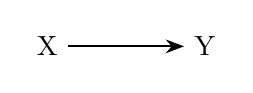
\begin{tikzpicture}[thick, >=Stealth]
    \node (x) at (-1, 0) {X};
    \node (y) at (1, 0) {Y};

    \draw[->] (x) -- (y);
  \end{tikzpicture}

  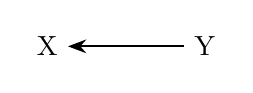
\begin{tikzpicture}[thick, >=Stealth]
    \node (x) at (-1, 0) {X};
    \node (y) at (1, 0) {Y};

    \draw[->] (y) -- (x);
  \end{tikzpicture}
\end{frame}

\begin{frame}{Confounding}
  \center
  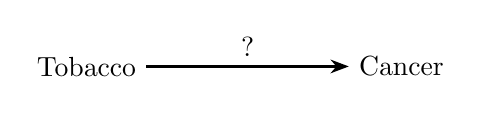
\begin{tikzpicture}[thick,>=Stealth]
    \node (tobacco) at (-2, 0) {Tobacco};
    \node (cancer) at (2,0) {Cancer};

    \draw[->] (tobacco) -- (cancer) node[midway, above] {?};
  \end{tikzpicture}
\end{frame}

\begin{frame}{Confounding}
  \center
  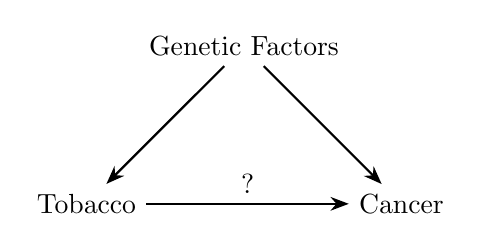
\begin{tikzpicture}[thick,>=Stealth]
    \node (tobacco) at (-2, 0) {Tobacco};
    \node (cancer) at (2,0) {Cancer};
    \node (genes) at (0, 2) {Genetic Factors};

    \draw[->] (tobacco) -- (cancer) node[midway, above] {?};
    \draw[->] (genes) -- (tobacco);
    \draw[->] (genes) -- (cancer);
  \end{tikzpicture}
\end{frame}

\begin{frame}
  \begin{center}
    Confounder (or Fork)

    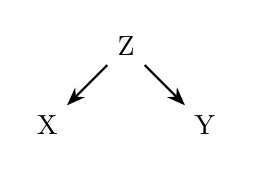
\begin{tikzpicture}[thick, >=Stealth]
        \node (x) at (-1, 0) {X};
        \node (y) at (1, 0) {Y};
        \node (z) at (0, 1) {Z};

        \draw[->] (z) -- (x);
        \draw[->] (z) -- (y);
    \end{tikzpicture}

  \end{center}
\end{frame}

\begin{frame}
\begin{center}
  \huge
  Collider

  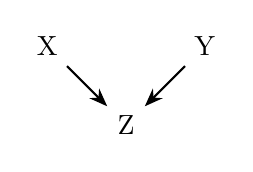
\begin{tikzpicture}[thick, >=Stealth]
    \node (x) at (-1, 0) {X};
    \node (y) at (1, 0) {Y};
    \node (z) at (0, -1) {Z};

    \draw[->] (x) -- (z);
    \draw[->] (y) -- (z);
  \end{tikzpicture}
\end{center}
\end{frame}

\begin{frame}
  \begin{block}{The Secret of Stats}
    \begin{enumerate}
    \item Generate some fake data (Gelman, McElreath)
    \item Make a statistical model
    \item Test if the model can recover parameters
    \item Use it on experimental data
    \end{enumerate}
  \end{block}
\end{frame}

\begin{frame}
  Further reading:
  \begin{itemize}
  \item Bayesian Methods for Hackers
  \item Statistical Rethinking
  \item The Book of Why
  \item Causal Inference In Statistics, a primer
  \end{itemize}
\end{frame}

\end{document}
